%%%%%%%%%%%%%%%%%%%%%%%%%%%%%%%%%%%%%%%%%
% Research Report Assignment Title Page 
% LaTeX Template
% Version 1.0 (06/03/16)
%
% This template has been downloaded from:
% http://www.LaTeXTemplates.com
%
% Original author: Francisco Maria Calisto
% WikiBooks (http://en.wikibooks.org/wiki/LaTeX/Title_Creation)
%
% License:
% CC BY-NC-SA 3.0 (http://creativecommons.org/licenses/by-nc-sa/3.0/)
% 
% Instructions for using this template:
% This title page is capable of being compiled as is. This is not useful for 
% including it in another document. To do this, you have two options: 
%
% 1) Copy/paste everything between \begin{document} and \end{document} 
% starting at \begin{titlepage} and paste this into another LaTeX file where you 
% want your title page.
% OR
% 2) Remove everything outside the \begin{titlepage} and \end{titlepage} and 
% move this file to the same directory as the LaTeX file you wish to add it to. 
% Then add \input{./title_page_1.tex} to your LaTeX file where you want your
% title page.
%
%%%%%%%%%%%%%%%%%%%%%%%%%%%%%%%%%%%%%%%%%
%\title{Title page with logo}
%----------------------------------------------------------------------------------------
%	PACKAGES AND OTHER DOCUMENT CONFIGURATIONS
%----------------------------------------------------------------------------------------

\documentclass[12pt]{article}
\usepackage[english]{babel}
\usepackage[utf8x]{inputenc}
\usepackage{amsmath}
\usepackage{graphicx}
\usepackage[colorinlistoftodos]{todonotes}
\usepackage{subcaption}

\begin{document}

\begin{titlepage}

\newcommand{\HRule}{\rule{\linewidth}{0.5mm}} % Defines a new command for the horizontal lines, change thickness here

\center % Center everything on the page
 
%----------------------------------------------------------------------------------------
%	HEADING SECTIONS
%----------------------------------------------------------------------------------------

% Name of your university/college
\textsc{\LARGE Instituto Superior T\'{e}cnico}\\[1.5cm]
% Major heading such as course name
\textsc{\Large ISR}\\[0.5cm]
% First Minor heading such as course title
\textsc{\large Report}\\[0.25cm]
% Second Minor heading such as course title
\textsc{\small Conceptual Model Milestone}\\[0.25cm]

%----------------------------------------------------------------------------------------
%	TITLE SECTION
%----------------------------------------------------------------------------------------

\HRule \\[0.5cm]
{ \large \bfseries First Surveys \& Prototypes}\\[0.25cm] % Title of your document
\HRule \\[0.5cm]
 
%----------------------------------------------------------------------------------------
%	AUTHOR SECTION
%----------------------------------------------------------------------------------------

\begin{minipage}{0.4\textwidth}
\begin{flushleft} \large
\emph{Author:}\\
Francisco Maria \textsc{Calisto} % Your name
\end{flushleft}
\end{minipage}
~
\begin{minipage}{0.4\textwidth}
\begin{flushright} \large
\emph{Coordinator:} \\
Jacinto \textsc{Nascimento} % Coordinator's Name
\end{flushright}
~
\begin{flushright} \large
\emph{Co-Coordinator:} \\
Daniel \textsc{Gon\c{c}alves} % Co-Coordinator's Name
\end{flushright}
\end{minipage}\\[2cm]

% If you don't want a supervisor, uncomment the two lines below and remove the section above
%\Large \emph{Author:}\\
%John \textsc{Smith}\\[3cm] % Your name

%----------------------------------------------------------------------------------------
%	DATE SECTION
%----------------------------------------------------------------------------------------

{\large 04/08/2016}\\[1cm] % Date, change the \today to a set date if you want to be precise

%----------------------------------------------------------------------------------------
%	LOGO SECTION
%----------------------------------------------------------------------------------------

% 
\includegraphics{ist-logo.png}\\[0.5cm] % Include a department/university logo - this will require the graphicx package

% 
\includegraphics{isr-logo.png}\\[0.5cm] % Include a department/university logo - this will require the graphicx package

\begin{figure}
\centering
\begin{subfigure}{.5\textwidth}
  \centering
  
\includegraphics[width=.5\linewidth]{isr-logo.png}
\end{subfigure}%
\begin{subfigure}{.5\textwidth}
  \centering
  
\includegraphics[width=.5\linewidth]{inesc-id-logo.png}
\end{subfigure}
\begin{subfigure}{.5\textwidth}
  \centering
  
\includegraphics[width=.25\linewidth]{ist-logo.png}
\end{subfigure}
\end{figure}
 
%----------------------------------------------------------------------------------------

\vfill % Fill the rest of the page with whitespace

\end{titlepage}

\section{Abstract}

Mammography is the primary method of image diagnosis used for screening and diagnosis of breast cancer, with an embodiment recommended image in several countries like Europe and the United States to use in screening programs. The implementation of digital technology caused changes in the practice of mammography, including the need to adapt quality control programs.

Our goal with this report is to start to characterising the current mammography technology in Portugal and practices in their use by professionals health involved. Finish on the level of harmonisation of practices in mammography in Portugal and compliance with international recommendations. Identify opportunities for optimisation to ensure the use of effectiveness and technologically safe.

The methodology followed here was the research and data collection on technology deployed, provided by government sources, mammography service providers and industry. Construction of surveys, oriented to the profile of radiologist physicians and some others clinical specialities with activity in digital mammography. The surveys were applied in providers selected as mammography services based on geographically location criteria, type of technology installed and profile of the institution.

\clearpage

\section{Introduction}

The technology for breast imaging has been the subject of major developments in the last decade with several multi-modalities (MRI and Ultrasound) to currently play a major role in disease breast management. Mammography (image produced with X-rays) is the main method used in the screening and Diagnosis of Breast Cancer signals, keeping the recommended imaging multi-modality for use in screening programs in several countries in Europe and the USA. The mammography limitations are known, specifically their limited specificity sensitivity and in the detection and characterisation of lesions, particularly in dense breasts and in young women. Studies on the effectiveness of the mammogram in women over 50 indicate sensitivity values between 68\% and 90\% and variable specificity between 82\% and 97\%.

The value of Ultrasonography (US) and Magnetic Resonance Imaging (MRI) is recognised as a complement to mammography. Computed Tomography (CT), Positron Emission Mammography (PEM) and Breast Scintigraphy (SPECT) are methods also used in the diagnosis and evaluation of breast pathology.

Digital technology mammography effectiveness has been proven in several clinical studies the last decade. Currently there are several options commercially available for digital mammography differ the detector characteristics acquisition system and image processing and its integration with source X-Ray.

In this report we intend to disclose some figures relating to clinical collaboration in the project and its objectives, showing preliminary results of the characterisation of the installed technology activities in the evaluated institutions and ongoing practices as a physicians sample.

It is an overall of the report objective to conclude on the level of harmonisation of practices in mammography in this physicians sample and study compliance with the international recommendations/guidelines. It also intends to identify opportunities to promote the quality of mammograms.

\clearpage

\section{Surveys}

Throughout the survey development were emerging doubts that prompted questions about points that would be clogged with the low-fidelity prototype. For a first sample of reasonability and report the quality of aid has been claimed to Doctor Cristina Ribeiro da Fonseca to help us validate the survey and some of the questions.

This first survey will be used to characterise the user of a mammography imaging multimodality interface being carried out in the framework of an innovative interface for monitoring and diagnosis of breast lesions and various medical imaging modalities. The questionnaire takes about 10 minutes and is divided into 9 short phases.

The first part is a simple description of what is the project and what the objectives to face are on the rest of the project.

Second part is made to understand the Doctor's profile where we ask questions like sex, age, etc. It is also in this section we try to understand a little of the professional profile that most mammography professionals have and in this way is questioned how long are medical functions prosecute, which sectors where the doctor works in that infrastructure and finally what specialty.

In the third part we characterise the clinical captivity by questions about it, the technological preferences, the clinical practice and its support for visualisation, tools, technologies and software of its medical units.

The fourth section aims to help us understand that training has the doctors working in the field. Asking if they have some kind of training in digital mammography and their views given the need to update knowledge in digital mammography and mammography certification in Portugal.

Section five makes some question of technical nature, here will be asked which mammographic image acquisition doses as well as knowledge of exposure/dose indicators to monitor the quality of the examination. It is also in this section that is asked the opinion of the physician to the impact of digital mammography in read/mammographic interpretation time.

\clearpage

Almost finally, the sections six, seven and eight question the opinions of physicians on technologies applied tools as Mammography, Ultrasound and Magnetic Resonance Imaging, respectively. In this sections we ask physicians about what frequency they use the next post-processing tools:

- Contrast;

- Contrast Inversion;

- Zoom;

- Pan;

- Fil;

- Crop;

- ROI;

- Annotation;

- Filters;

- Histogram;

- 3D Reconstruction;

- CAD;

This will bring us the information about the most useful tools to our User Interface and what are the priorities, since the order of appearance tools is important to physicians when time is a requirement to them.

Finally in the last section, the ninth, the issue of digital over the analog model with questions in the framework of improvements that brought digital face to analog and what it is covered.

\clearpage

\section{Low-Fidelity Prototypes}

During weeks we began transforming our discussion based and theoretical ideias into a conceptual model interface elements and workflows. We started with low-fidelity paper mock-ups since they let us easily and on a cheap way to create experimental interfaces and modify the structure of the elements.

Using the common material supplies like paper, markers, index cards, scissors and post-its, we sketched the first screens and elements structure, including menus, options and tools. The paper mock-up with its handwritten text, crooked lines, and last-minute corrections wasn't very neat but was enough to the user test physicians participants for what the basic structure of information and preferences look like.

\clearpage

% Commands to include a figure:
\begin{figure}[!hbt]
\centering
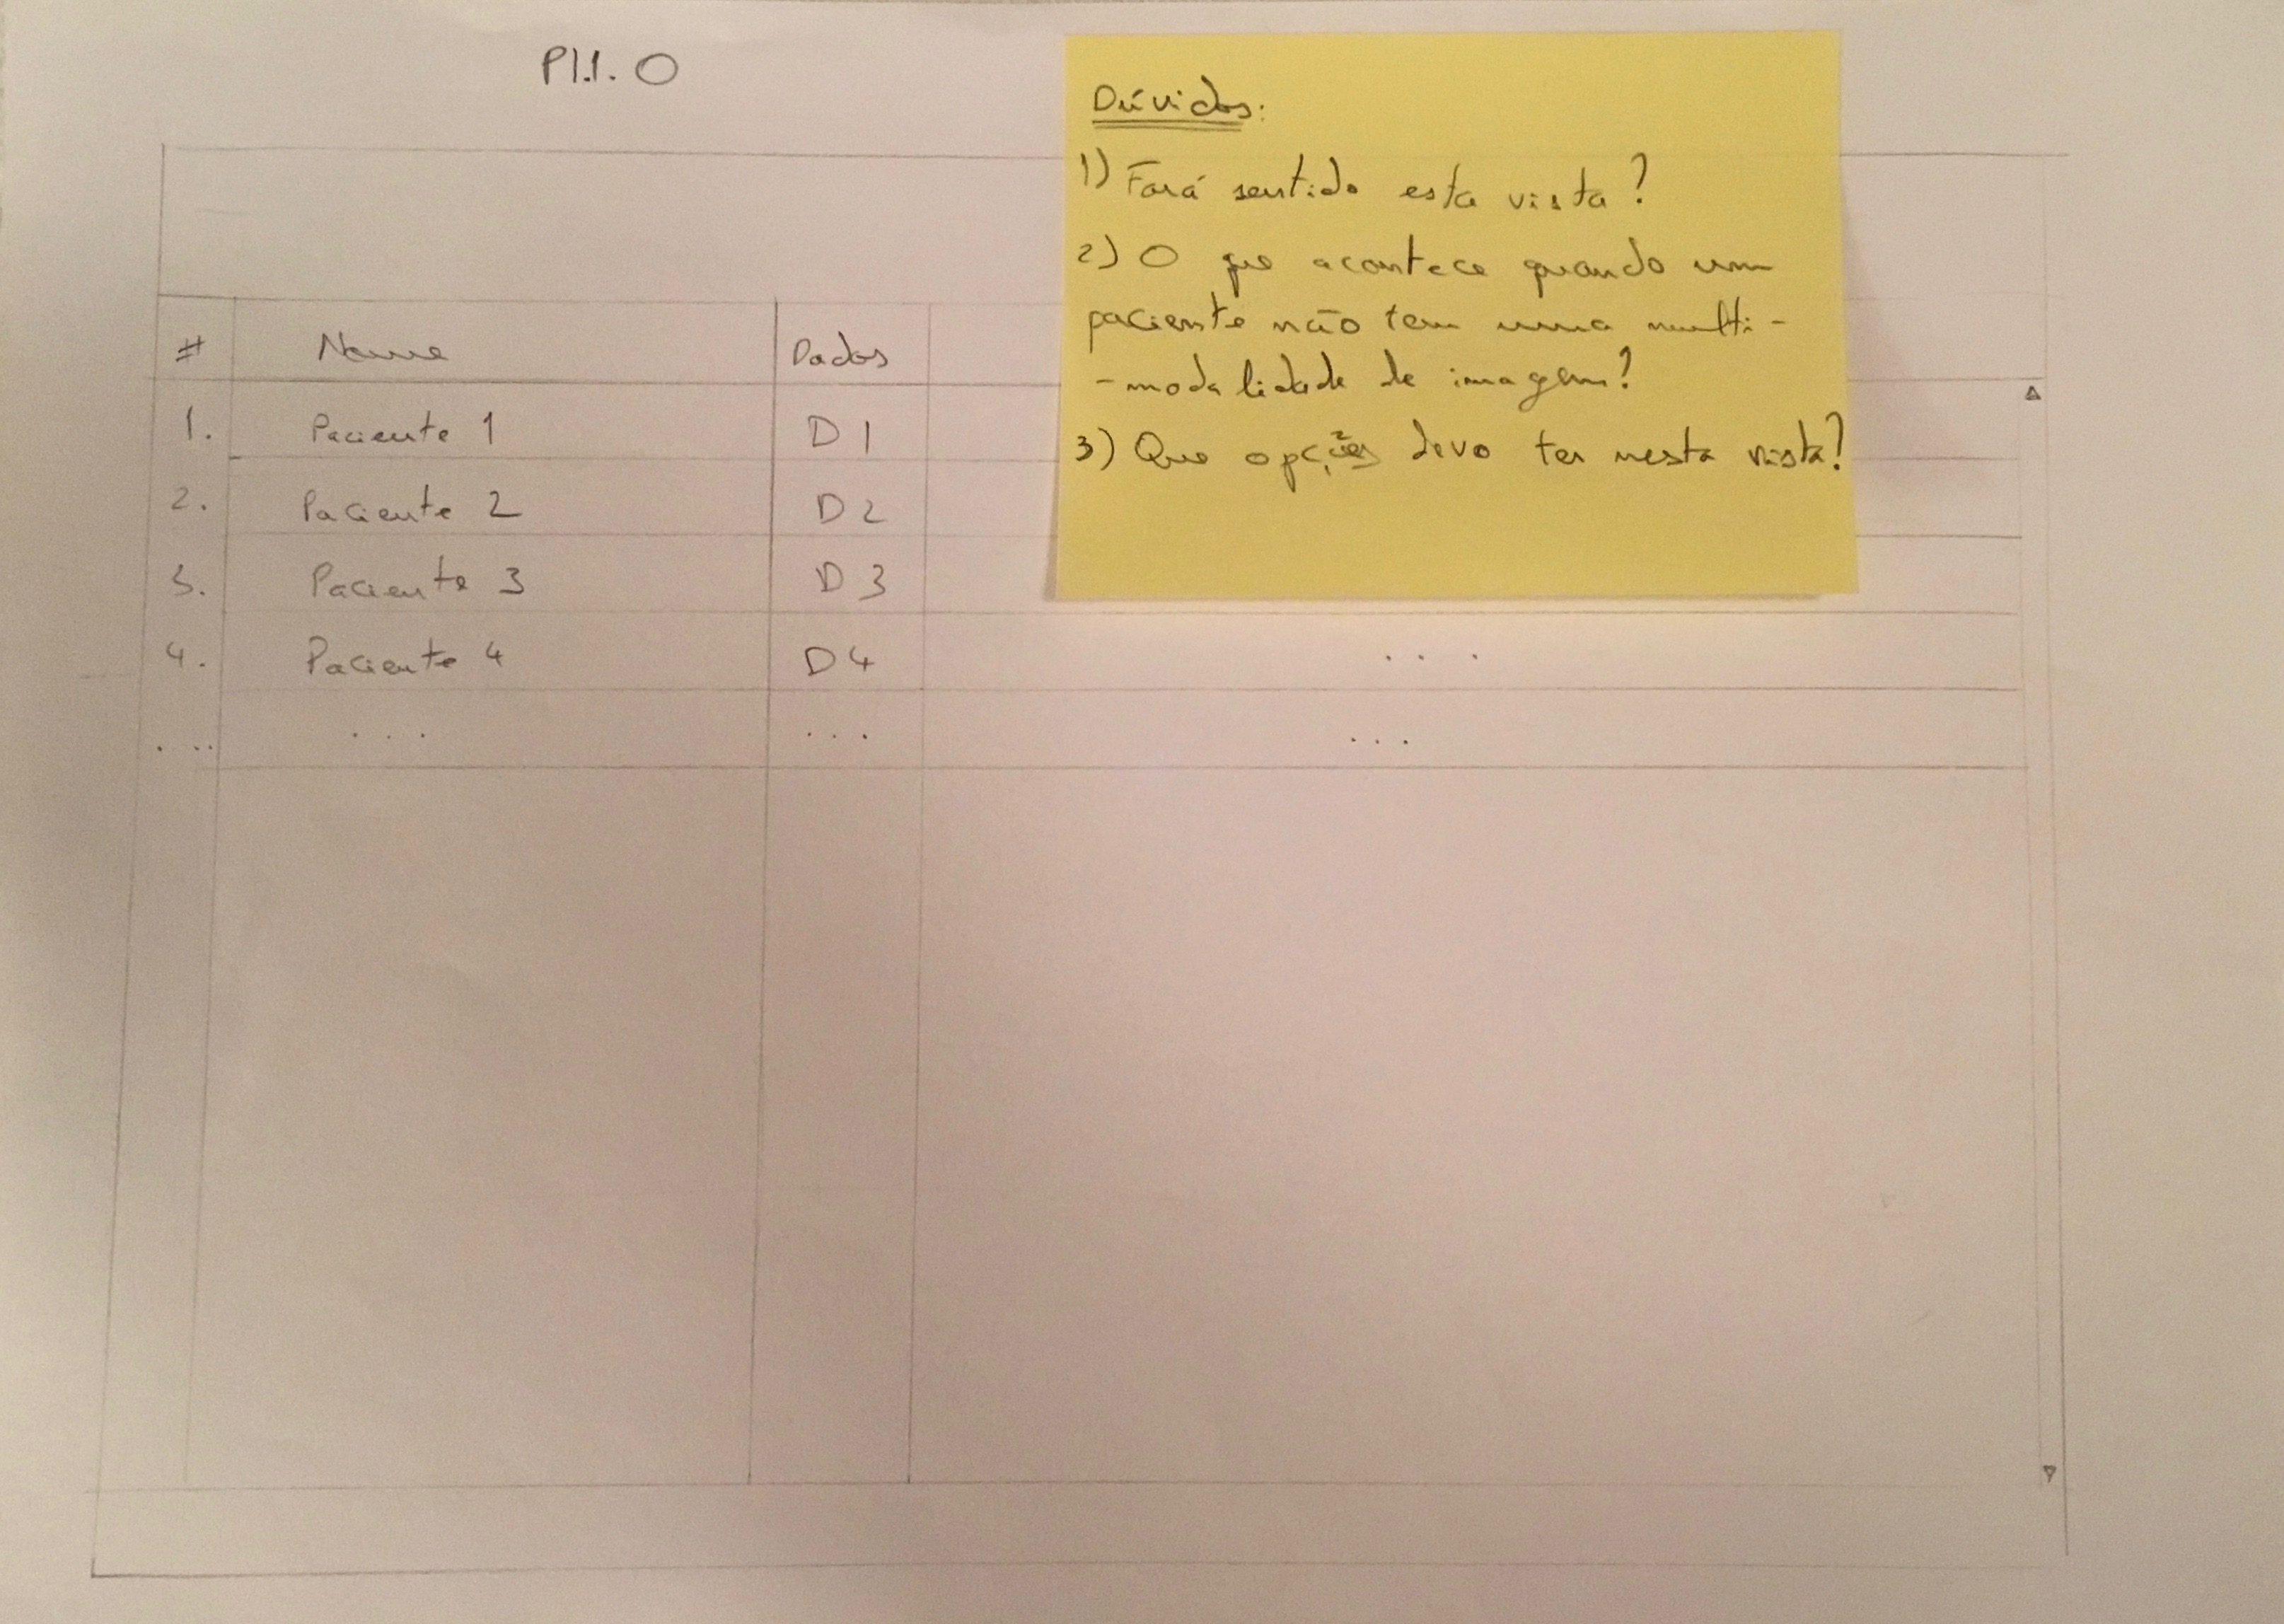
\includegraphics[width=1.00\textwidth]{p110.png}
\caption{\label{fig:P 1.1.0}Patients List.
}
\end{figure}

Our first screen (Figure 2) will show the user the first screen of the log, this screen is important to us since is the open window of the user interface and it is the first impact and how the physician will choose the patient. Even this is not our responsibility it is important to prototype this first screen to understand the usability and interaction between the screens.

\clearpage

% Commands to include a figure:
\begin{figure}[!hbt]
\centering
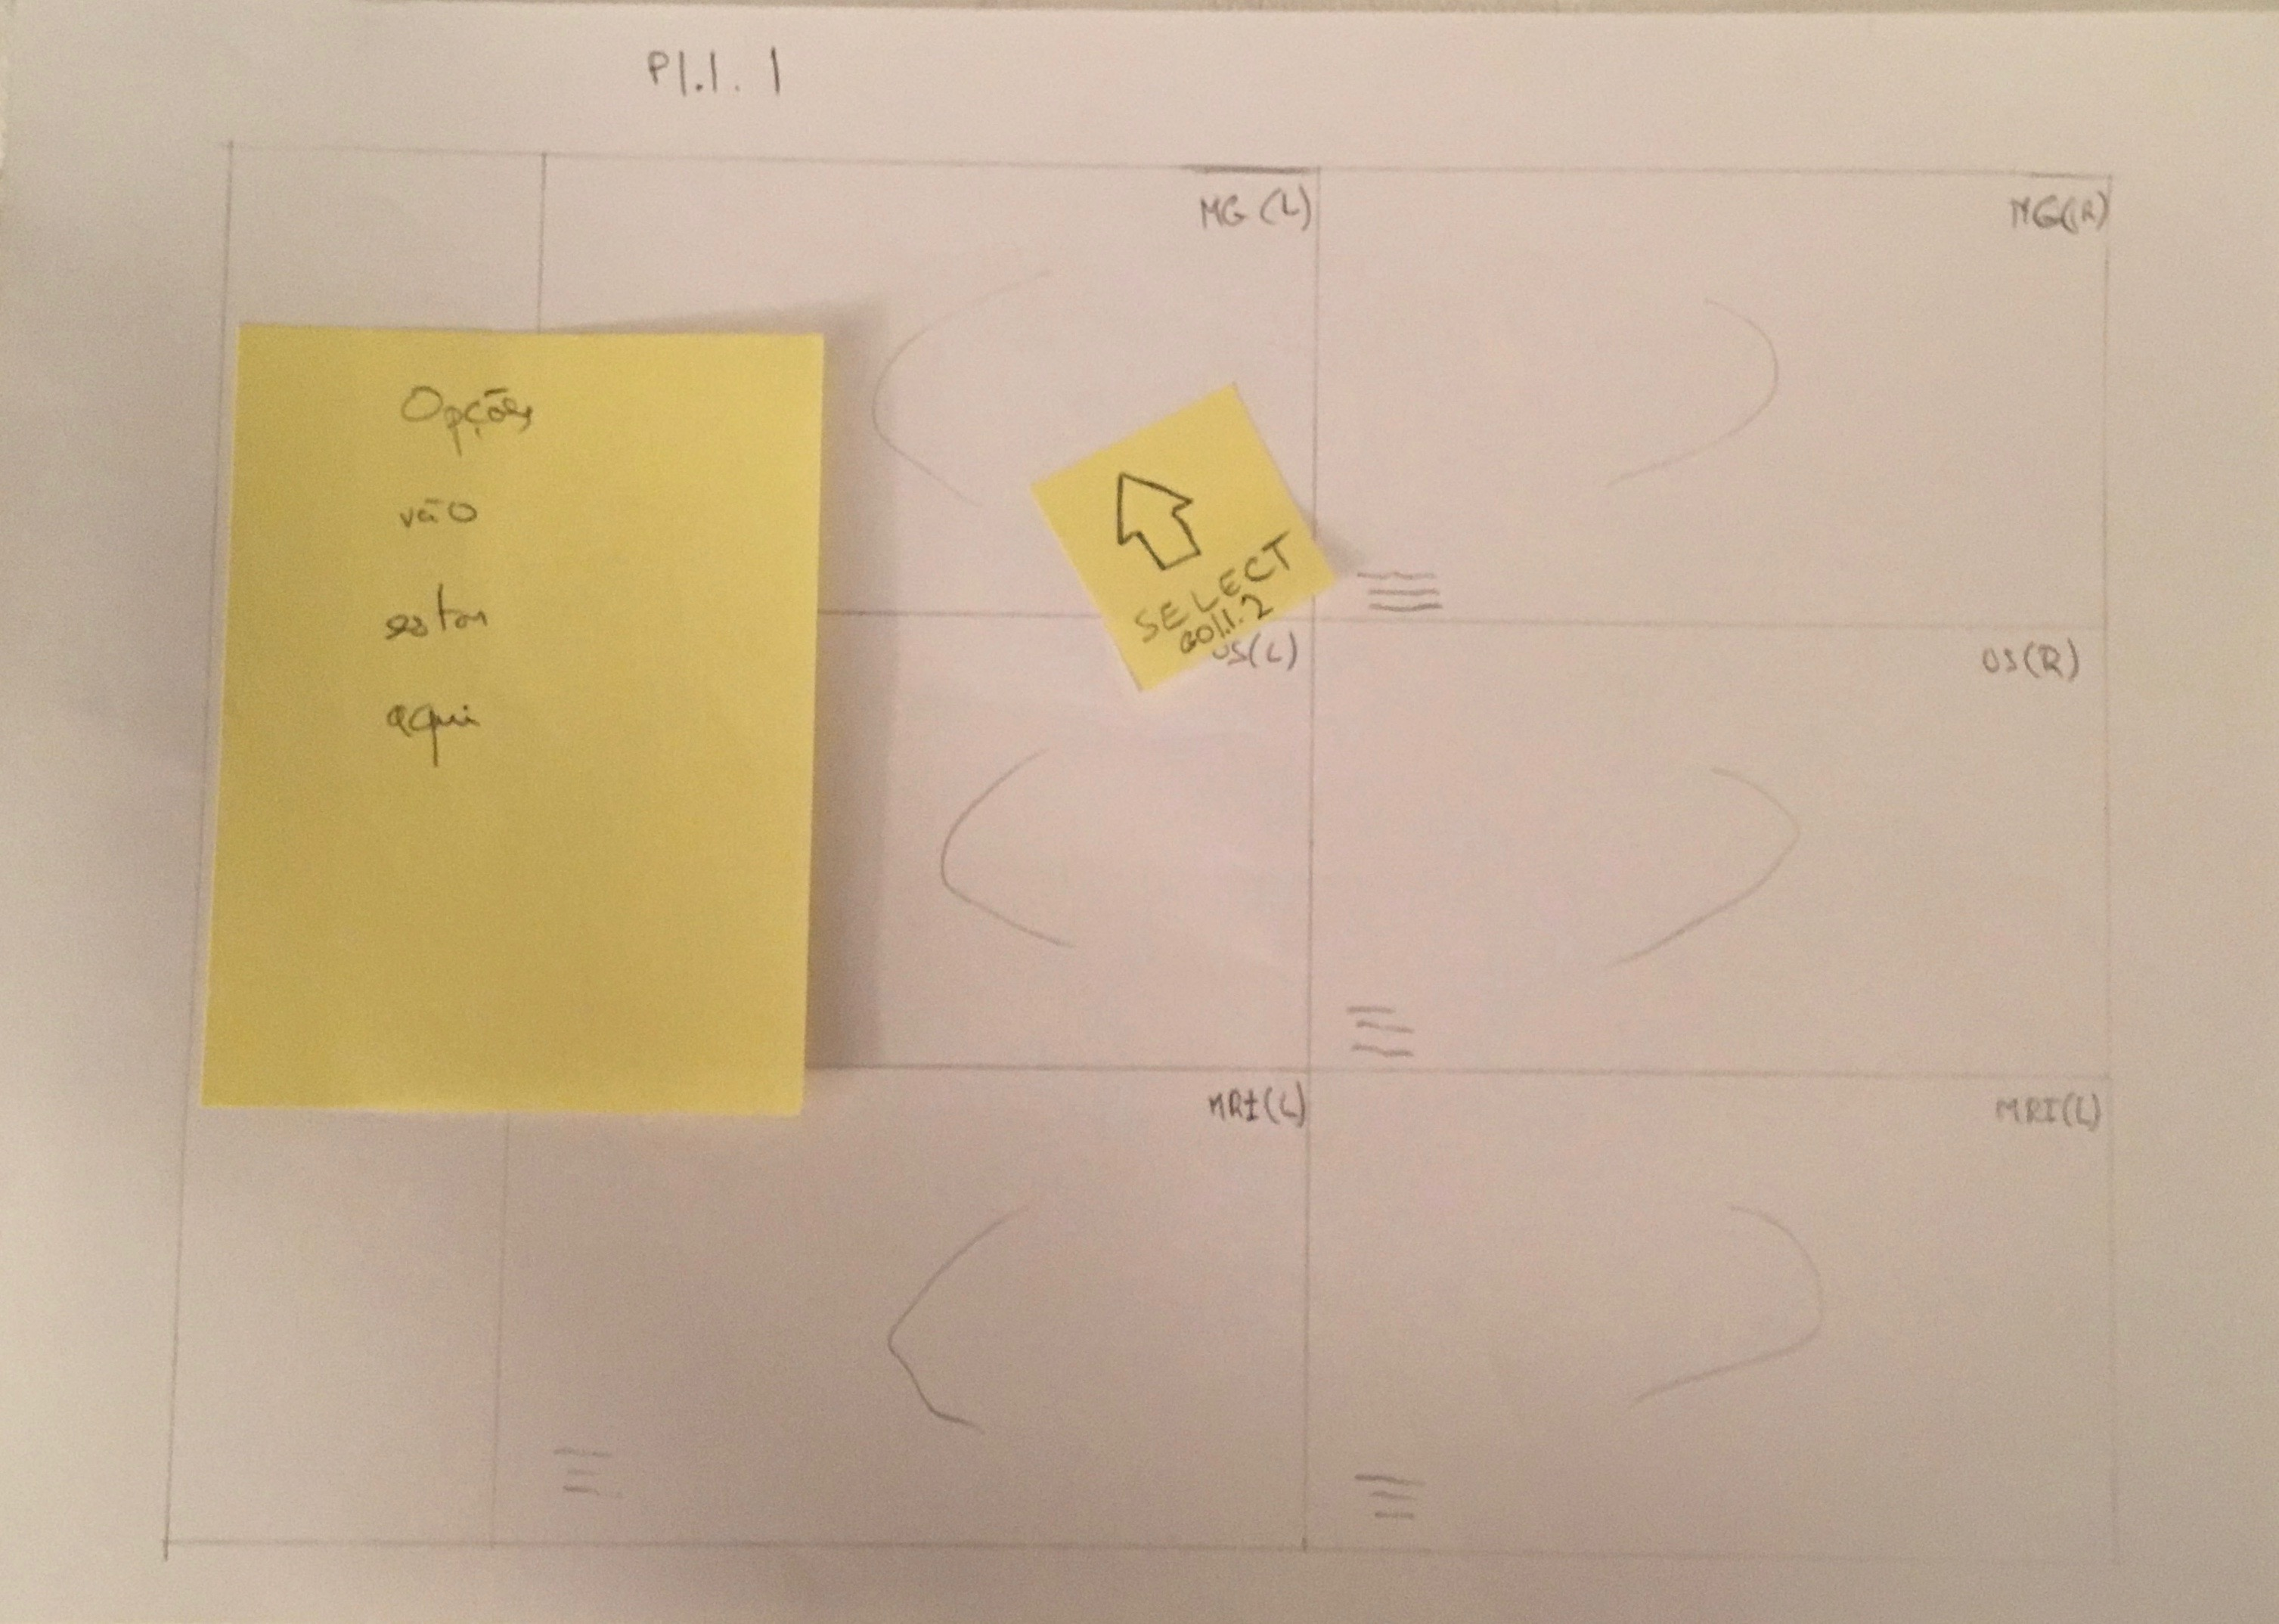
\includegraphics[width=1.00\textwidth]{p111.png}
\caption{\label{fig:P 1.1.1}SELECT Breast.
}
\end{figure}

On this screen (Figure 3) we validate how the multi-modality of image should be organised throw the screen. We also understand here where options should be and how the user interact with this options as follow the left click selection to have the entire view of a breast.

\clearpage

% Commands to include a figure:
\begin{figure}[!hbt]
\centering
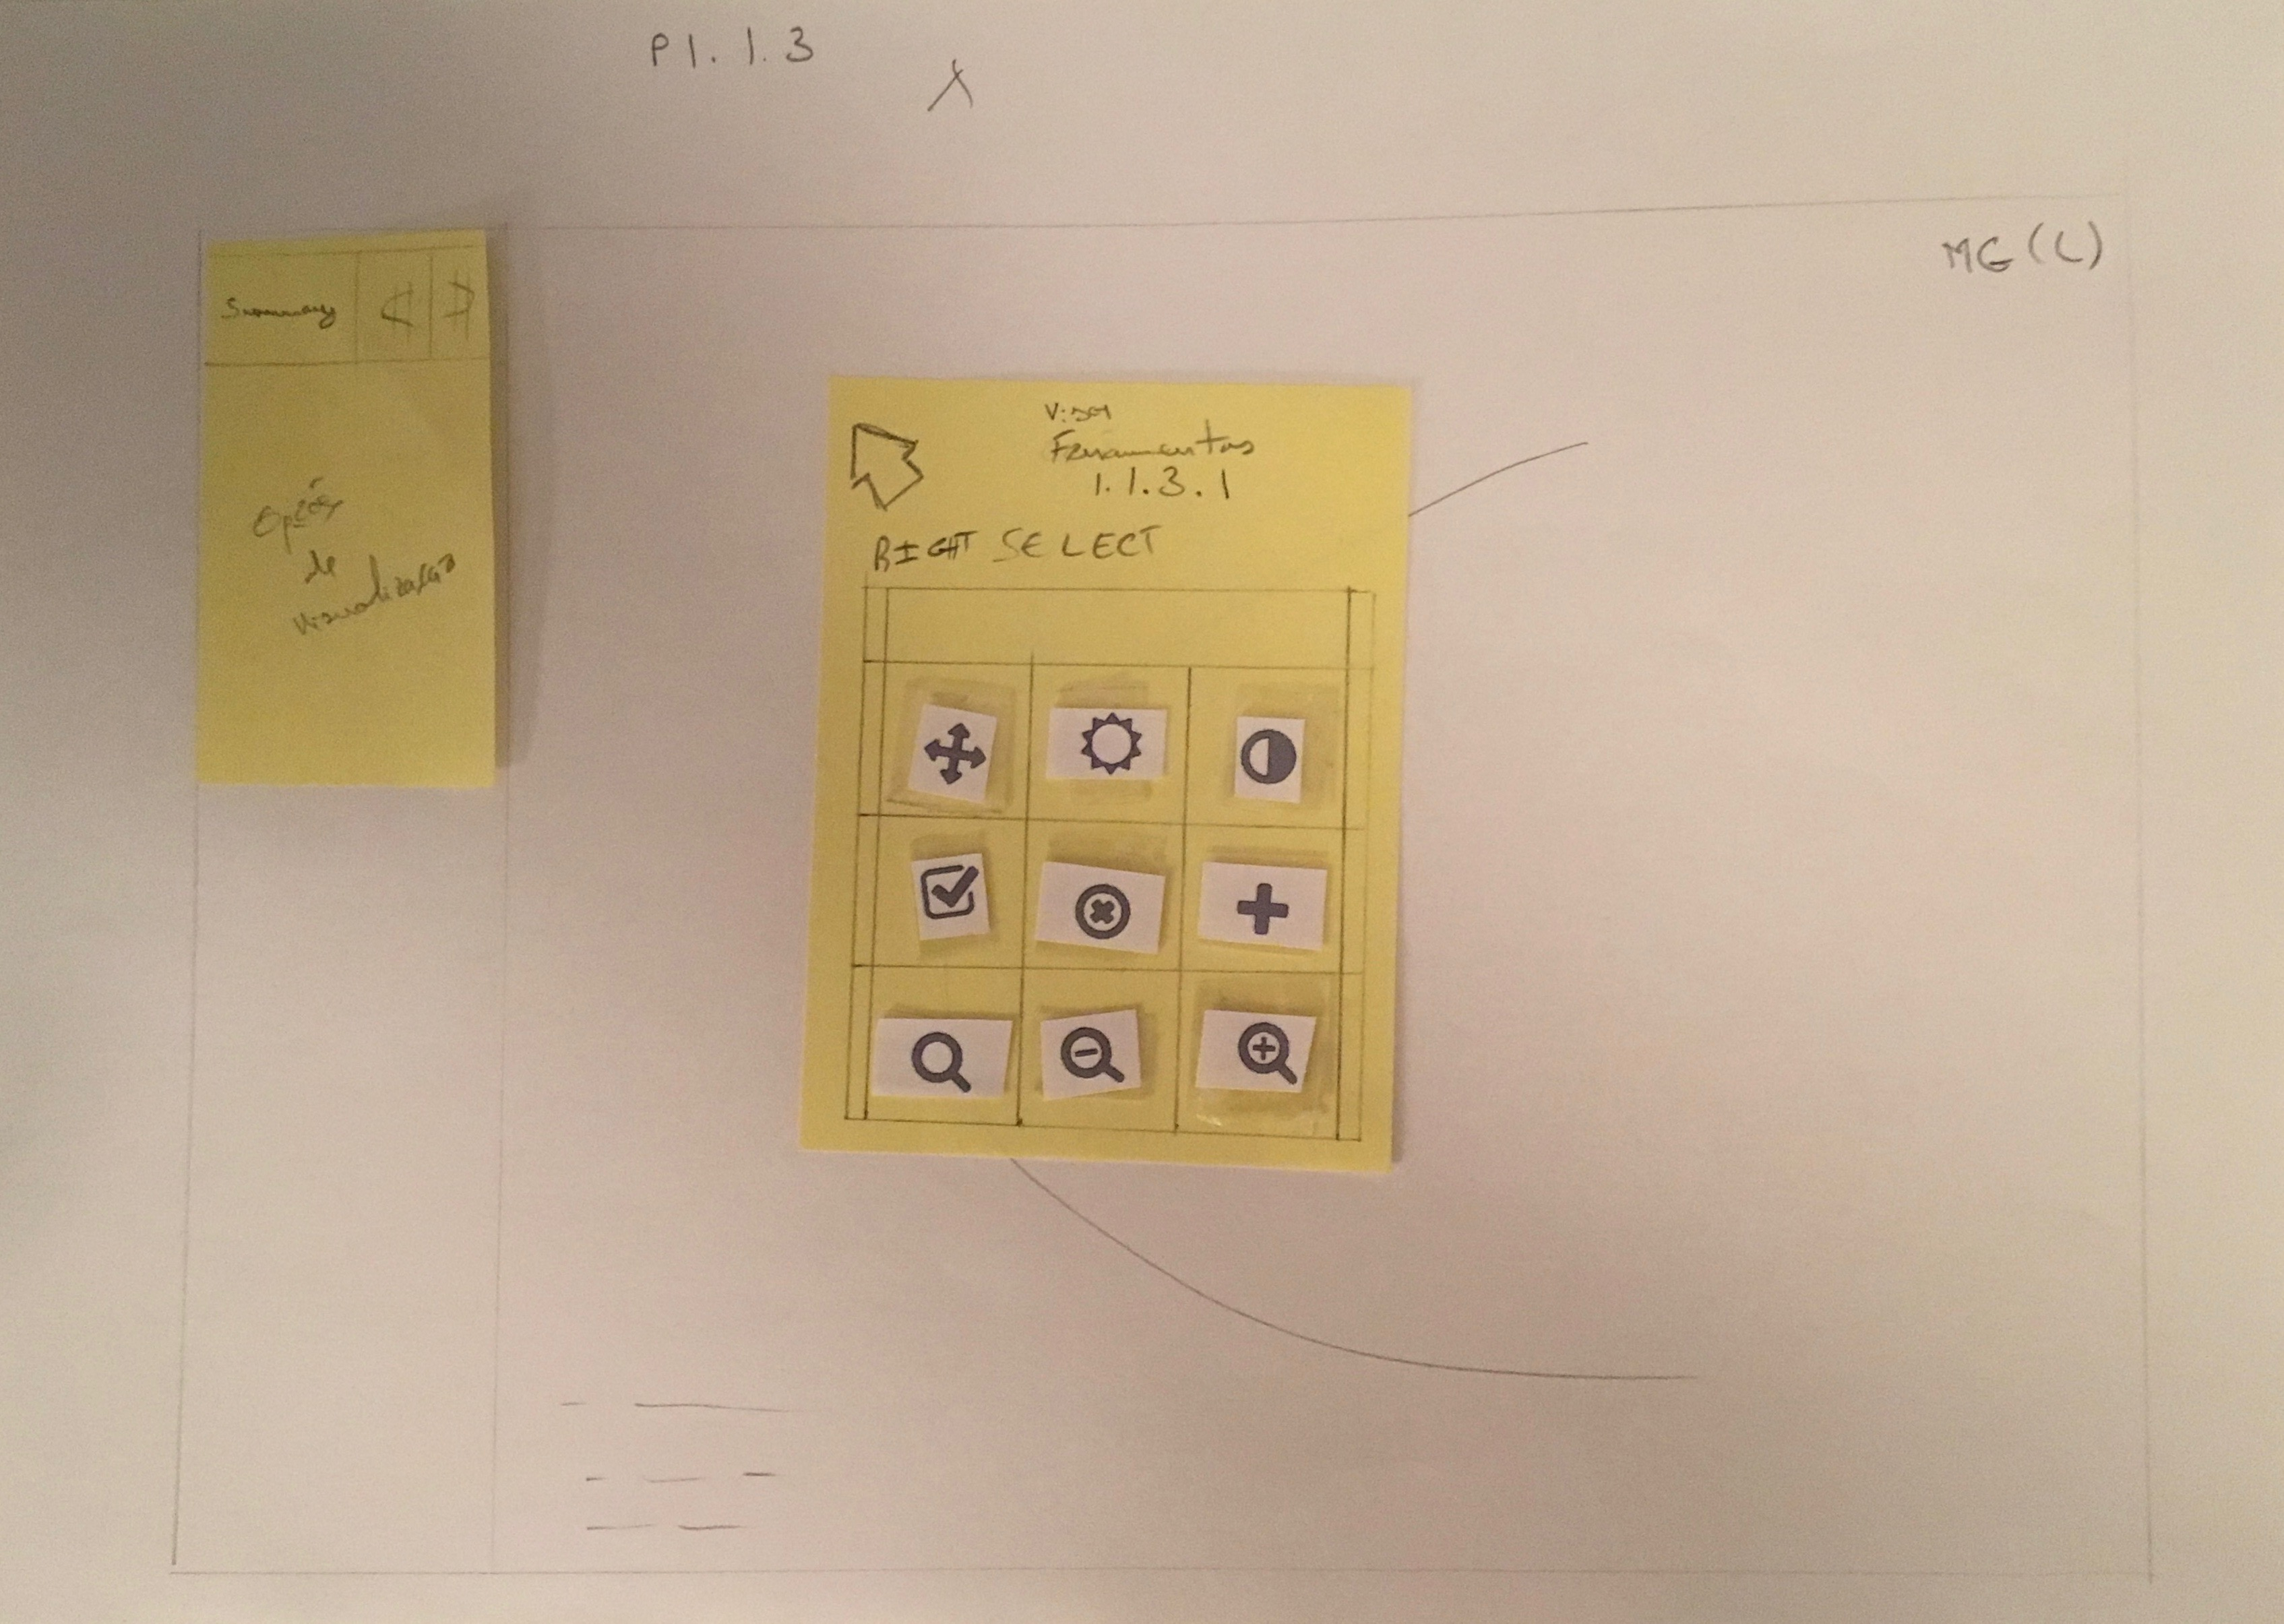
\includegraphics[width=1.00\textwidth]{p113.png}
\caption{\label{fig:P 1.1.3}RIGHT SELECT Options.
}
\end{figure}

A RIGHT SELECT Option seems to be the most common way to activate a tool box and as far as we understand it might be the best choice. It can increase the number of clicks but on the other hand will decrease time, for this reason is a better throughput requirement since physicians give more value to time against number of clicks.

\clearpage

% Commands to include a figure:
\begin{figure}[!hbt]
\centering
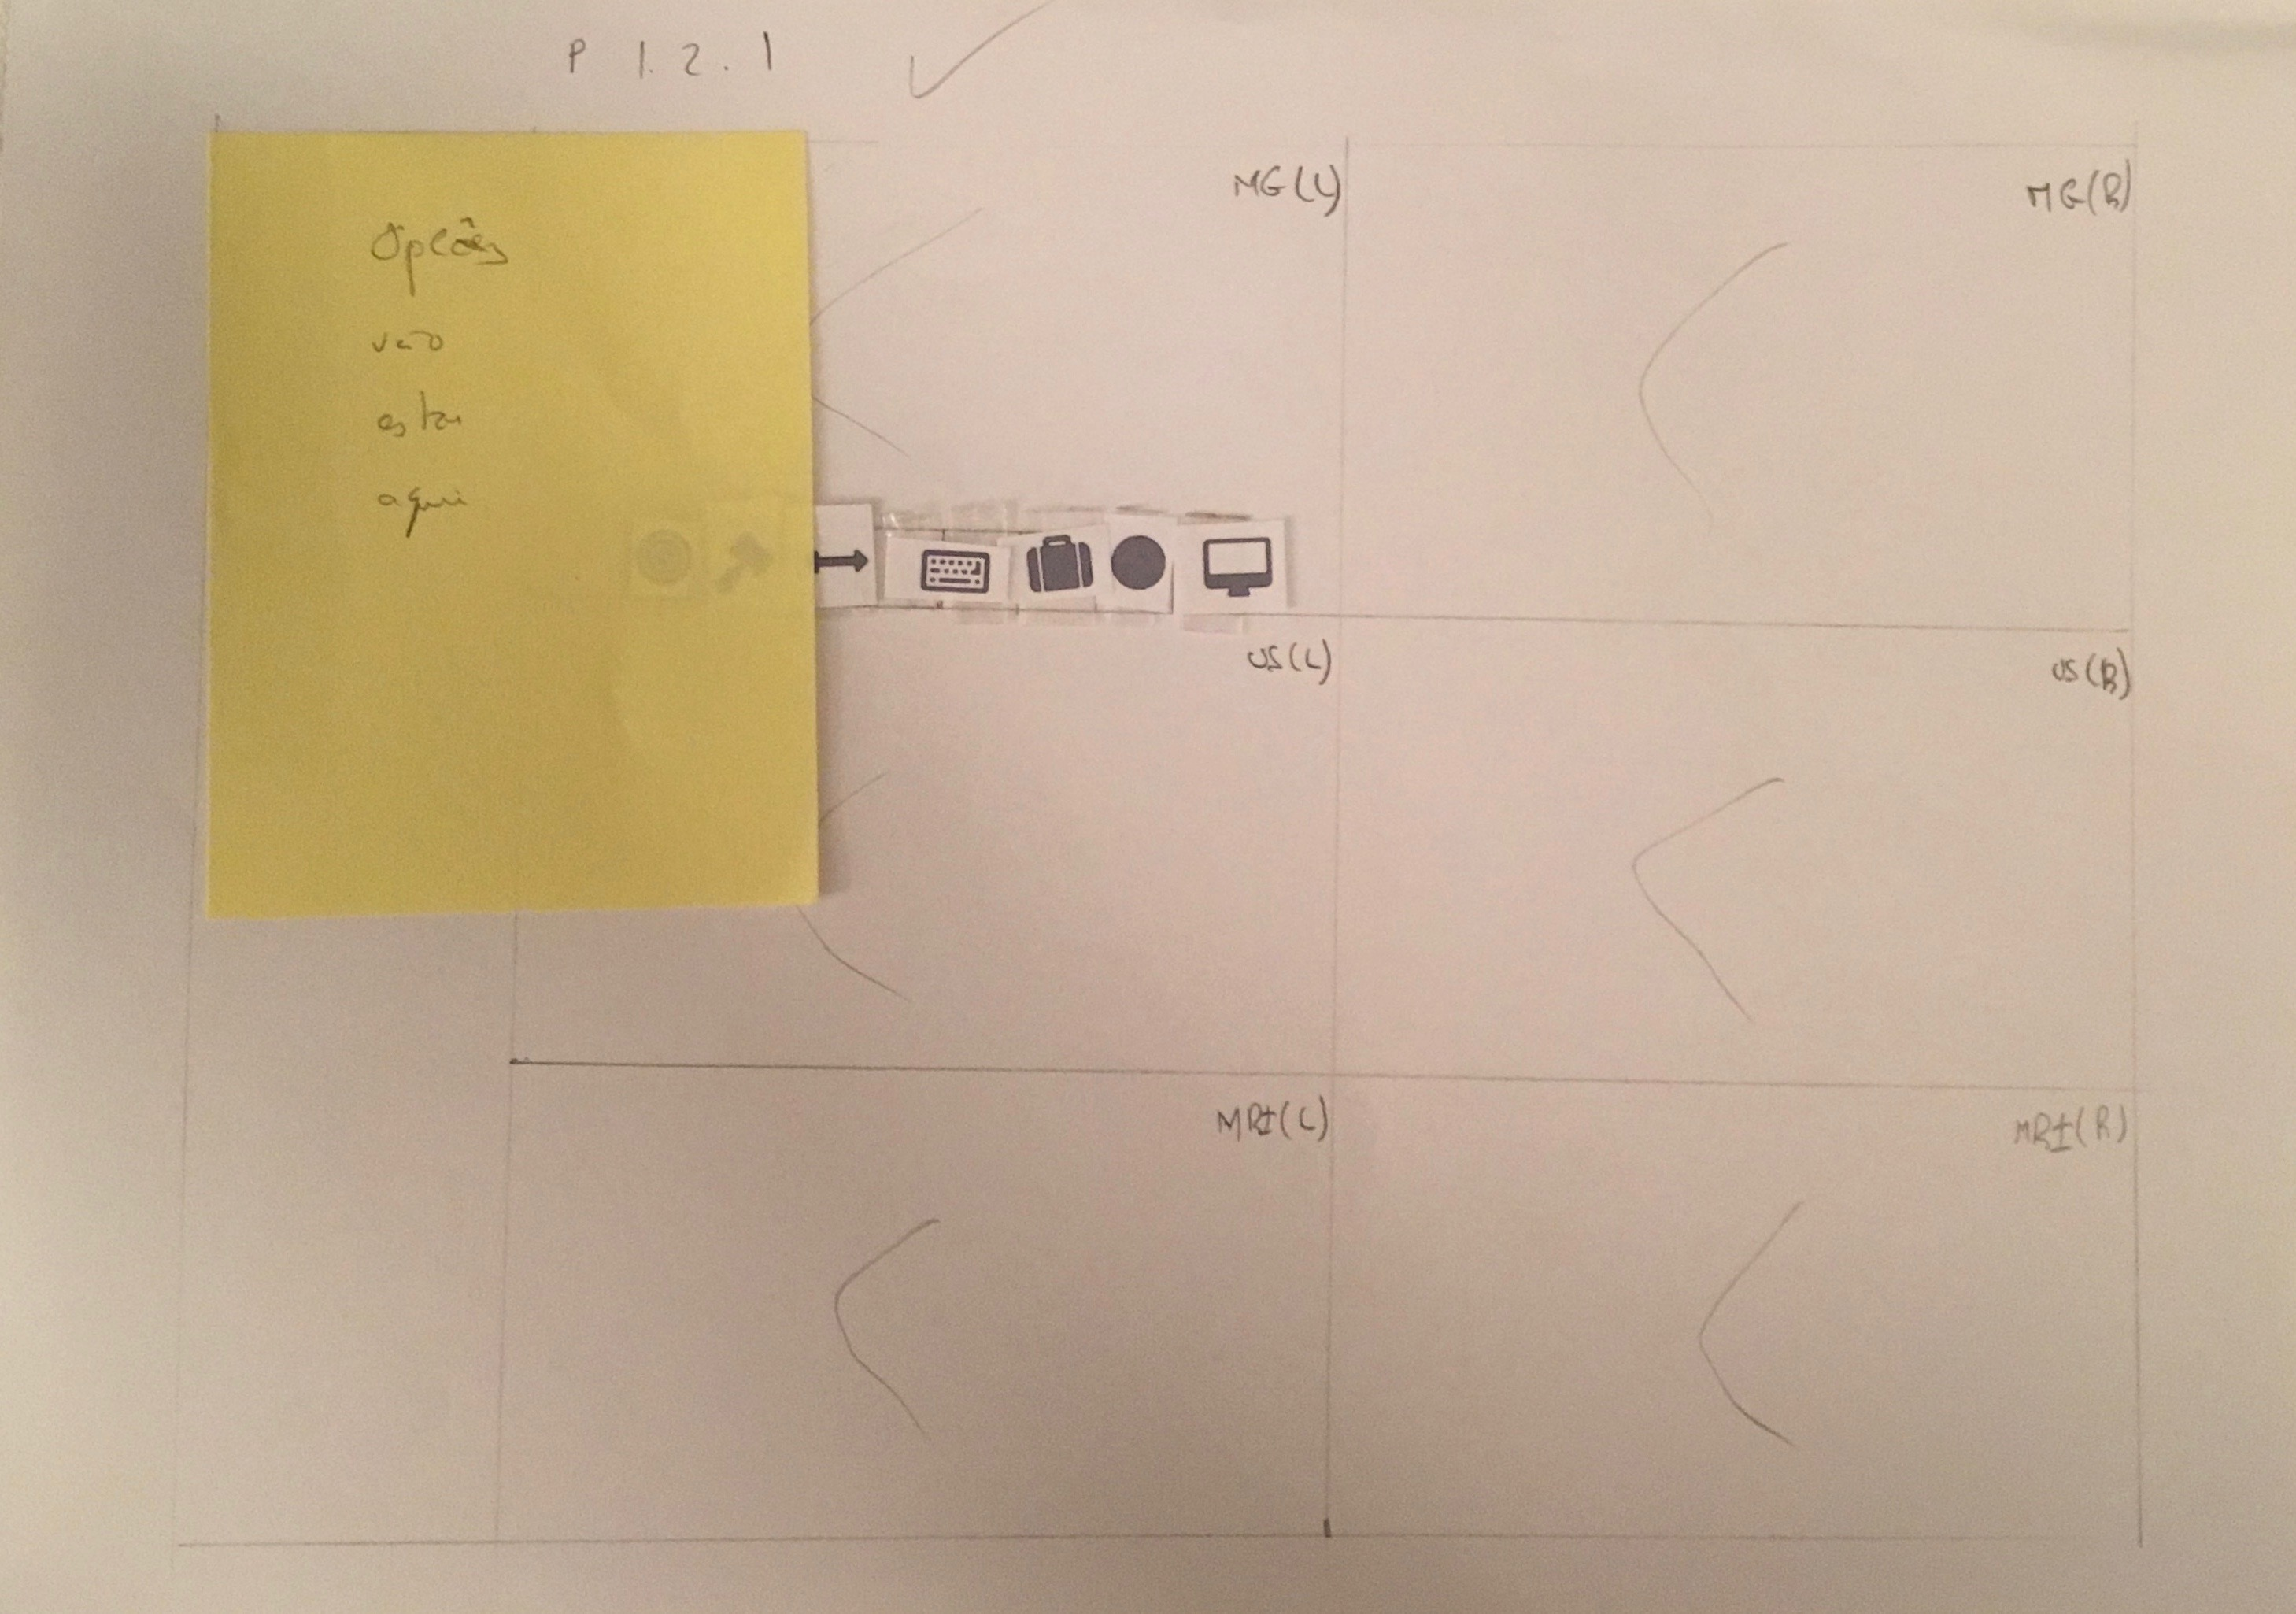
\includegraphics[width=1.00\textwidth]{p121.png}
\caption{\label{fig:P 1.2.1}Bottom Options.
}
\end{figure}

This screen (Figure 5) will show us other way to organise the tool box as we can see here we will have each small breast screen a bottom tool box. This minifies the number of clicks but we doubt it will increase the time to click.

\clearpage

% Commands to include a figure:
\begin{figure}[!hbt]
\centering
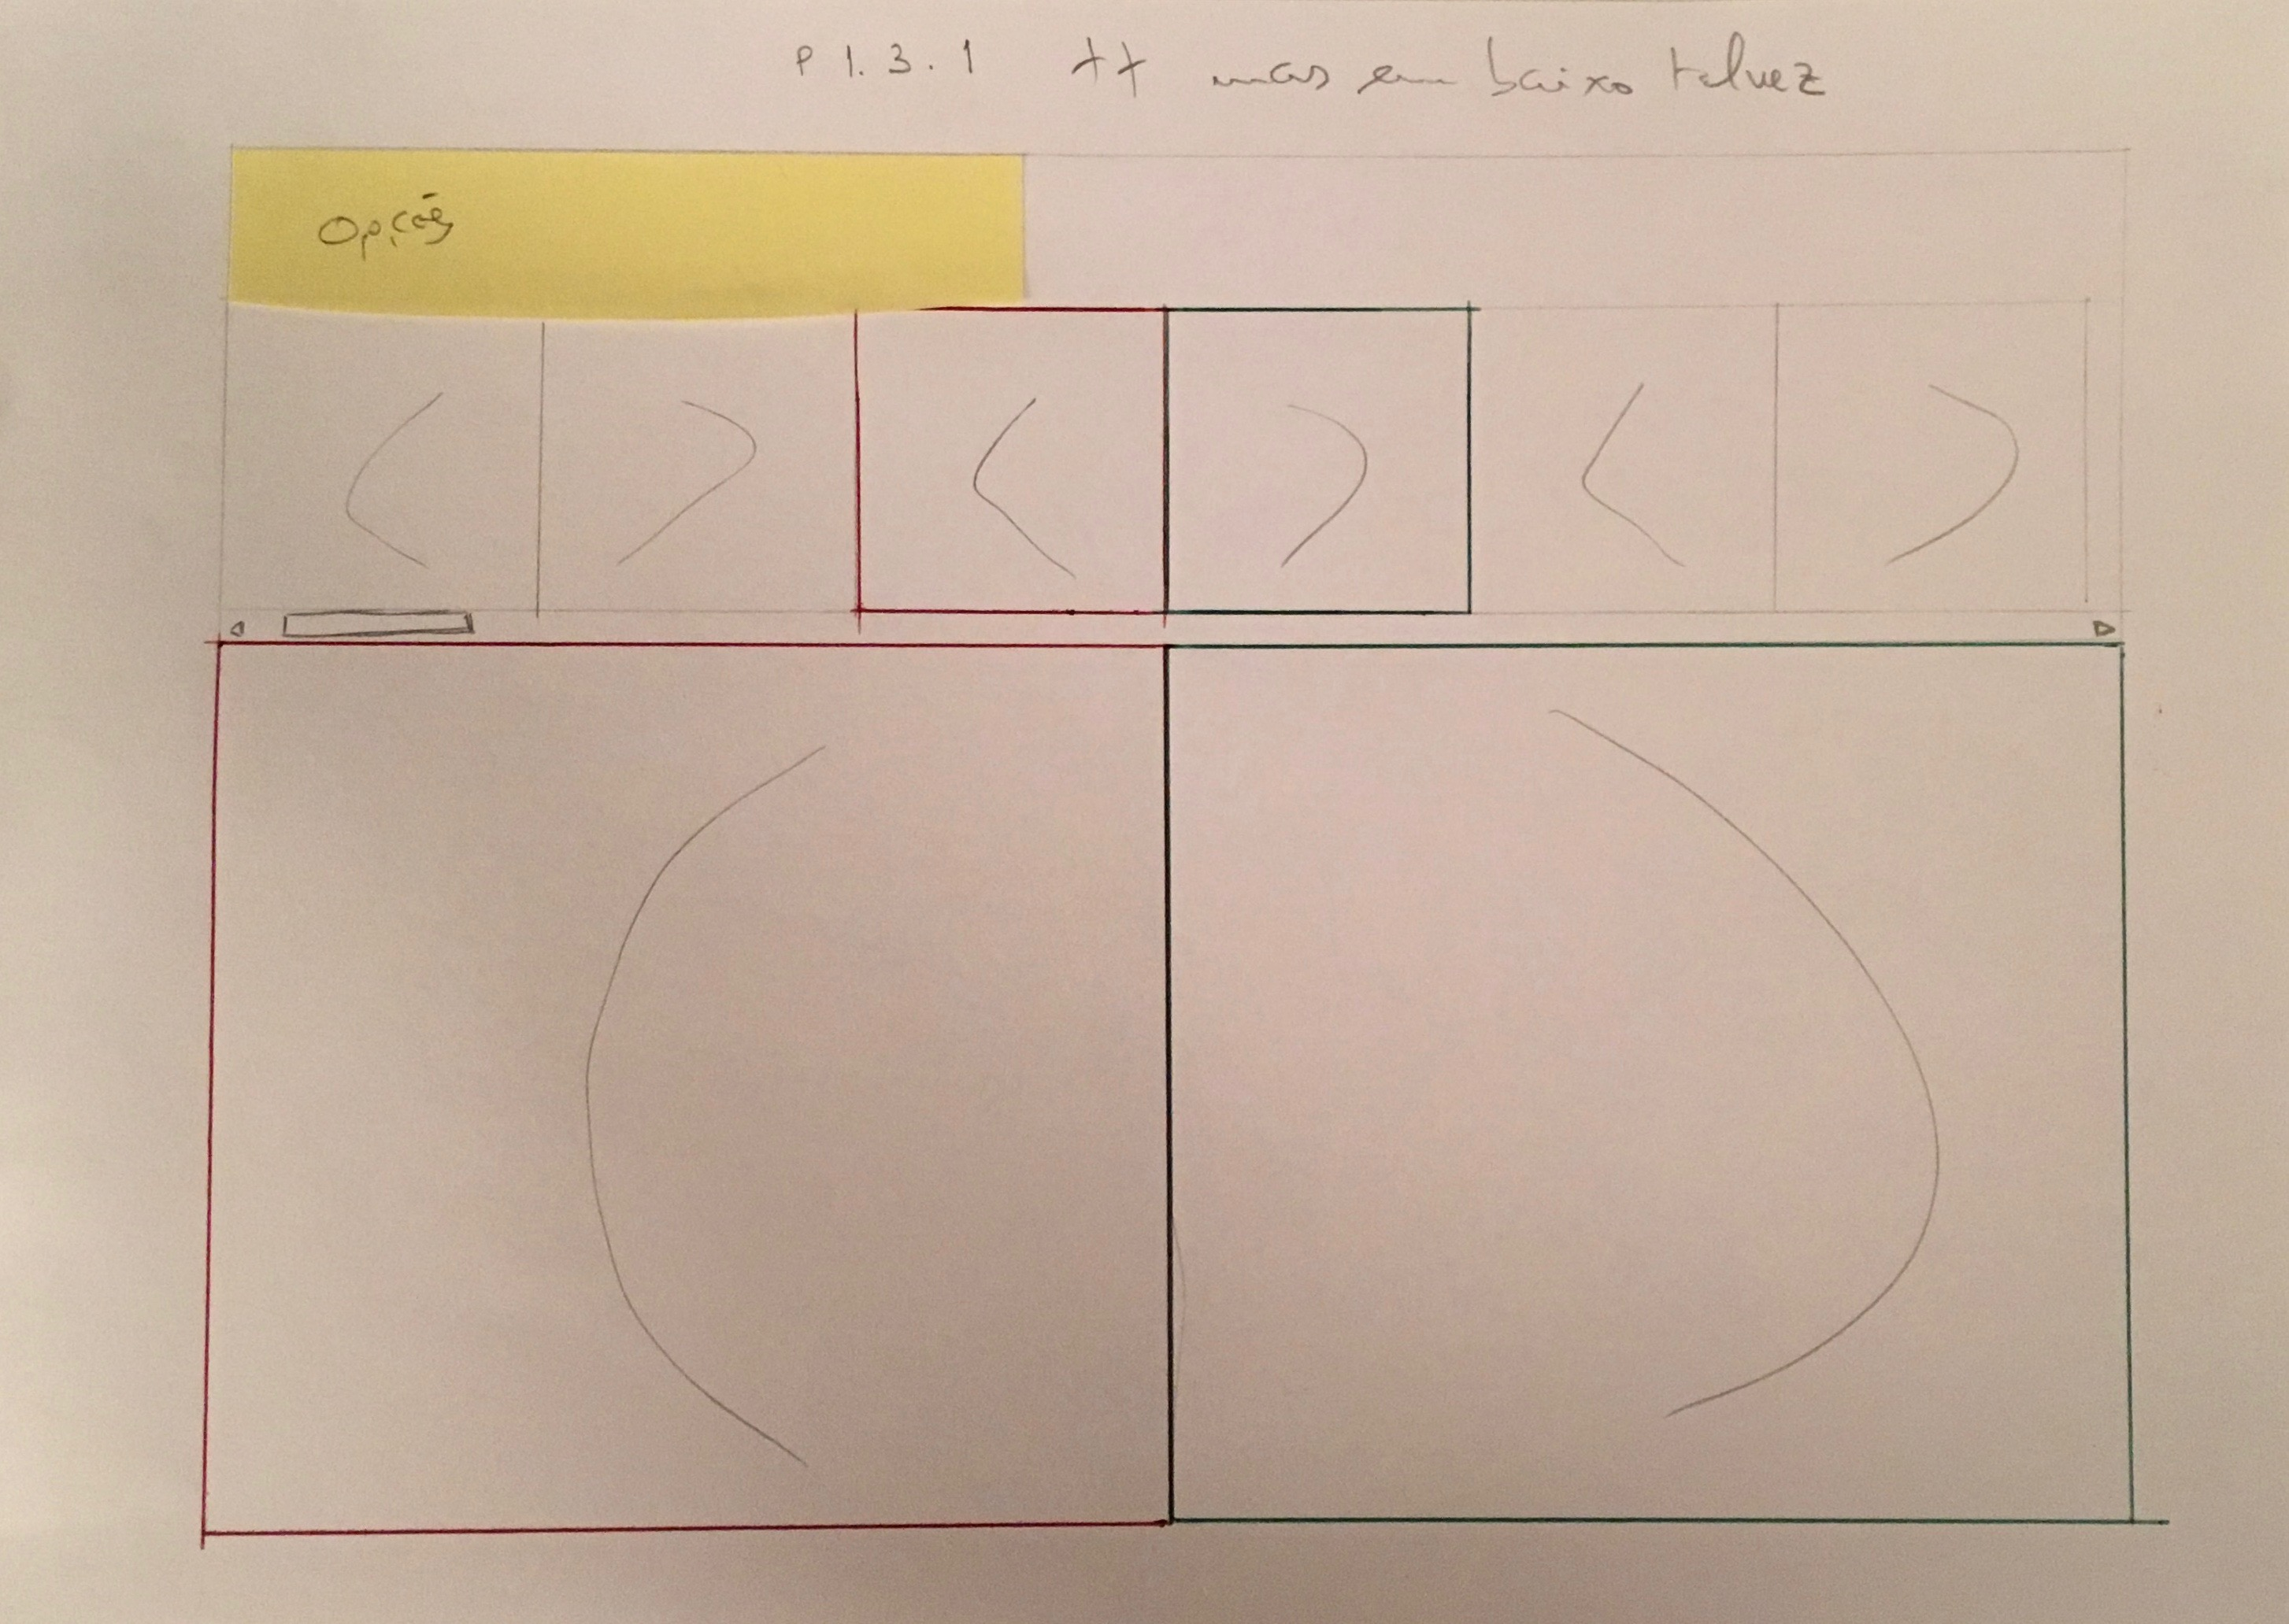
\includegraphics[width=1.00\textwidth]{p131.png}
\caption{\label{fig:P 1.3.1}Horizontal Breast Set.
}
\end{figure}

Horizontal Breast Set (Figure 6) is one of the options that we show to physicians evaluate how they feel more comfortable with. It seems to us the most intuitive way to organize the breast set of elements but is where we loose space since we only have a good two breast screen width, however, it might be better to have just two but with a viable size relatively to more breast on the screen but with a low width.

Again, for us it seems to be the better choice on a horizontal vs vertical of the breast set of options.

\clearpage

% Commands to include a figure:
\begin{figure}[!hbt]
\centering
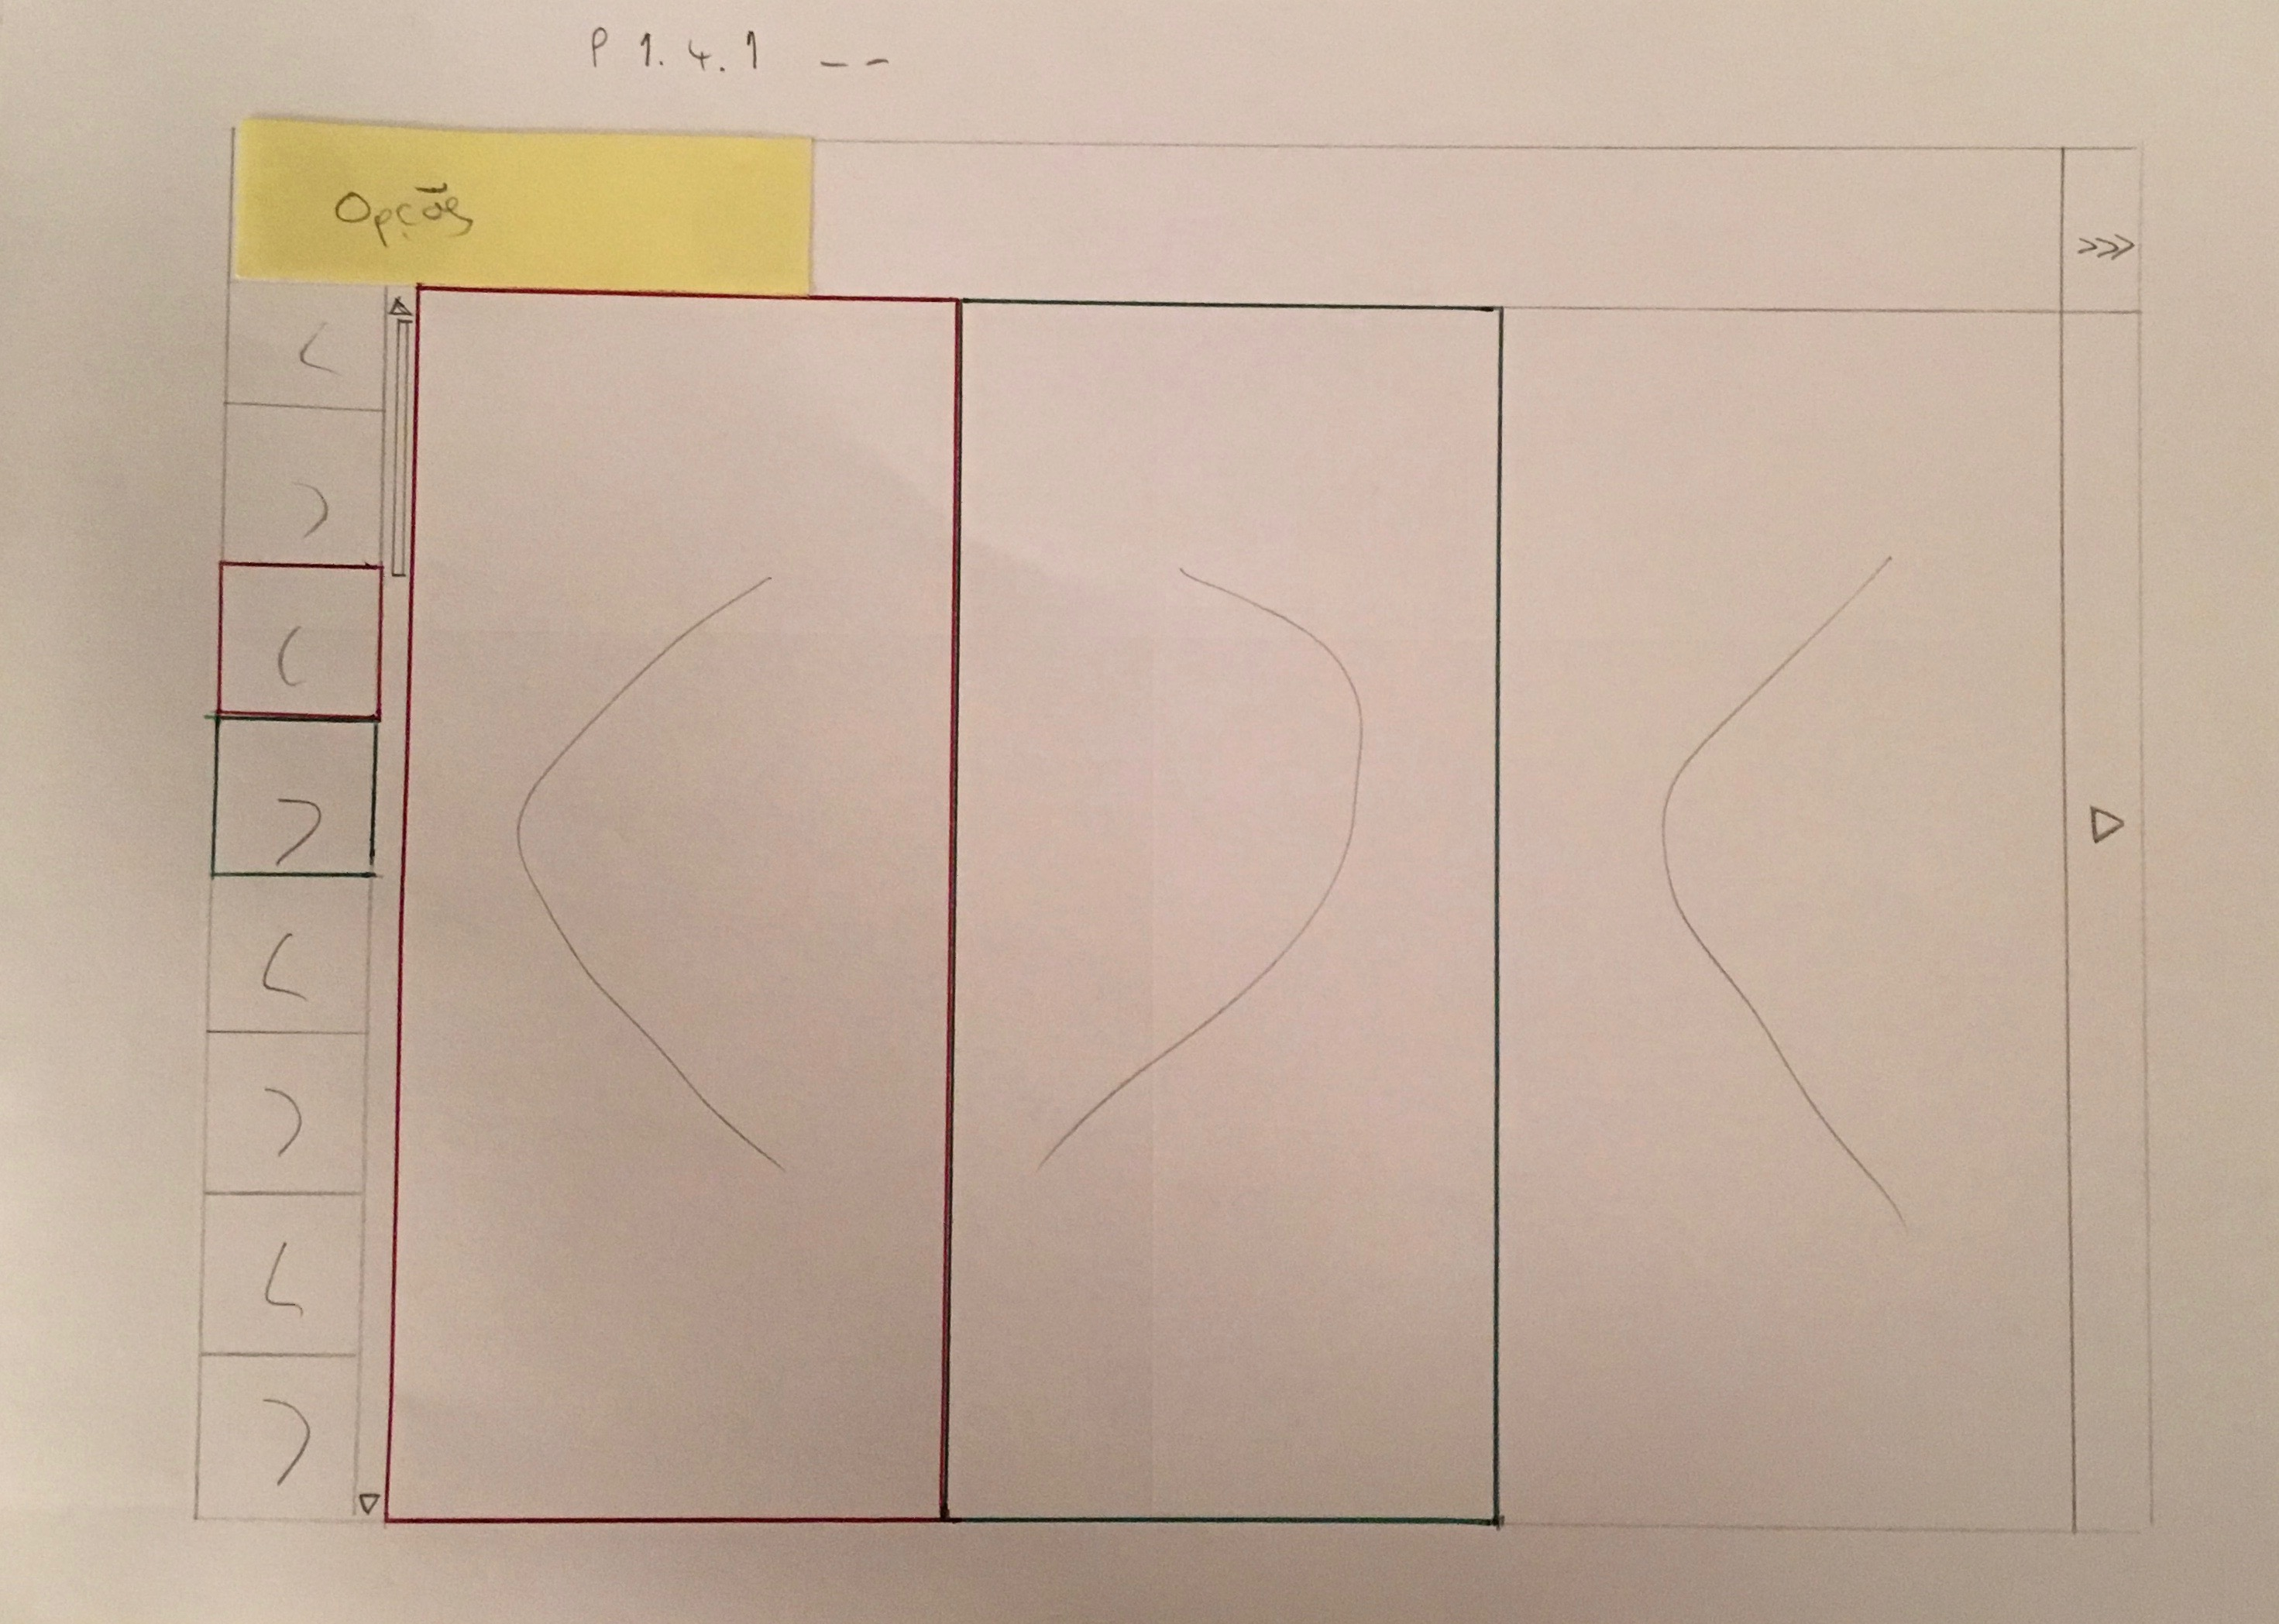
\includegraphics[width=1.00\textwidth]{p141.png}
\caption{\label{fig:P 1.4.1}Vertical Breast Set.
}
\end{figure}

Vertical Breast Set (Figure 7) is our second option that we show to physicians evaluate how they feel more comfortable with. We stress again the fact that this is might not be the best choice since we loose intuitive power, however we increase the number of breast on the screen and the number of sets on the sides of the screen since we can play here against the width and height.

\clearpage

\section{Conclusions}

Our current analysis and examples have shown how experience surveys and prototypes has contributed to real develop projects. By helping to develop understanding about the essence or essential factors of an existing experience, surveys and prototypes simulates important aspects of the whole or parts of the relationships between people and machine as they unfold over time. In exploration and evaluation of ideas surveys and prototypes can provide inspiration, confirmation or rejection of ideas based upon the quality of experience they engender.

At first surveys will give us the understanding of what requirements we should lead and what are the priorities. It also make us understand our target user (physicians), how they think, feel, how they understand the environment and how they work. Requirements can be hard to validate but a survey is a first approach from many to understand what questions we can do and how to do it. Is an important and cheap phase of the process that give us good guaranteers of what will be the final requirements and what the user wants and needs.

On the other hand, prototypes while it creates only approximate and partial simulations of the real experiences others will have, brings a subjective richness to bear on design problems. It is an approach that, we believe, will benefit from more conscious attention and deliberate experimentation.

Finally, we come back to the point that people's experiences with CAD and medical systems are a complex integration of physicians and circumstantial factors. Physicians will have experiences with things we develop, whether we intend them or not, and in ways that we cannot hope entirely to predict. Nevertheless, understanding, exploring and communicating the experiential aspects of design ideas are central activities in design.

\clearpage

\begin{thebibliography}{}
\bibitem{}
\end{thebibliography}




\end{document}
